% $Header: /cvsroot/latex-beamer/latex-beamer/solutions/conference-talks/conference-ornate-20min.en.tex,v 1.6 2004/10/07 20:53:08 tantau Exp $

\documentclass[trans]{beamer}
\usepackage{etex}
\newcommand\orh{\mbox{ ; }}
% This file is a solution template for:

% - Talk at a conference/colloquium.
% - Talk length is about 20min.
% - Style is ornate.



% Copyright 2004 by Till Tantau <tantau@users.sourceforge.net>.
%
% In principle, this file can be redistributed and/or modified under
% the terms of the GNU Public License, version 2.
%
% However, this file is supposed to be a template to be modified
% for your own needs. For this reason, if you use this file as a
% template and not specifically distribute it as part of a another
% package/program, I grant the extra permission to freely copy and
% modify this file as you see fit and even to delete this copyright
% notice.
%\usepackage{xcolor}
\usepackage{graphicx}
\usepackage{array}
\usepackage[all]{xy}
%\usepackage{theapa}
\usepackage{tikz}
\usetikzlibrary{shapes.geometric}
\usetikzlibrary{shadows}
\usetikzlibrary{positioning}
\usepackage{algorithm}
%\usepackage{algorithmic}
\usepackage{algpseudocode}
\usepackage{natbib}
\usepackage{apalike}
\mode<presentation>
{
%  \usetheme{AnnArbor}
%  \usetheme{Antibes}
%  \usetheme{Bergen}
%  \usetheme{Berkeley}
%  \usetheme{Berlin}
%  \usetheme{Boadilla}
%  \usetheme{boxes}
%  \usetheme{CambridgeUS}
%  \usetheme{Copenhagen}
%  \usetheme{Darmstadt}
%  \usetheme{default}
%  \usetheme{Dresden}
%  \usetheme{Frankfurt}
%  \usetheme{Goettingen}
%  \usetheme{Hannover}
%  \usetheme{Ilmenau}
%  \usetheme{JuanLesPins}
%  \usetheme{Luebeck}
%  \usetheme{Madrid}
%  \usetheme{Malmoe}
%  \usetheme{Marburg}
%  \usetheme{Montpellier}
%  \usetheme{PaloAlto}
%  \usetheme{Pittsburgh}
%  \usetheme{Rochester}
%  \usetheme{Singapore}
%  \usetheme{Szeged}
%  \usetheme{Warsaw}
  \usetheme{PLP}

%\usecolortheme{lily}%
  % or ...

  \setbeamercovered{transparent}
  % or whatever (possibly just delete it)
}


\usepackage[english]{babel}
% or whatever

%\usepackage[latin1]{inputenc}
% or whatever

\usepackage{times}
\usepackage[T1]{fontenc}
% Or whatever. Note that the encoding and the font should match. If T1
% does not look nice, try deleting the line with the fontenc.
\newcommand{\myalert}[1]{{%\color{red}
 #1}}
\newcommand{\fluffy}{\mathit{fluffy}}
\newcommand{\bdd}[2]
{
\begin{center}
\begin{tikzpicture}
[every node/.style={font=\scriptsize,minimum height=0.5cm,minimum width=0.5cm},x=2cm,y=1.2cm,rounded corners=2mm,zeroarrow/.style = {-stealth,dashed},
  onearrow/.style = {-stealth,solid},
  c/.style = {circle,draw,solid,minimum width=2em,
        minimum height=2em},
  r/.style = {rectangle,draw,solid,minimum width=2em,
        minimum height=2em}]
%[place/.style={shape=ellipse}]
%,draw=blue!50,fill=blue!20,thick,inner sep=0pt,minimum size=6mm},

\node[c] (X11) at (0,1) {#1};
   \node[c] (X21) at (1,1.5) {#2};
   \node[r] (final-one) at (2,0.5) {1};
   \node[r] (final-zero) at (2,1.5){0};
\node[] (lX11) at (0,0) {#1};
   \node (lX21) at (1,0) {#2};


   \path[onearrow,bend right=20] (X11) edge (final-one) ;
   \path[onearrow,bend right=20] (X21) edge   (final-one) ;

%      \draw[onearrow] (X11) -- (final-one);
%   \draw[onearrow] (X21) -- (final-one);

   \path[zeroarrow,bend left=20] (X11) edge  (X21) ;
   \path[zeroarrow,bend left=20] (X21) edge  (final-zero) ;
%
%   \draw[zeroarrow] (X11) -- (X21);
%   \draw[zeroarrow] (X21) -- (final-zero);
%
%\node (root) at ( 0,1) {};
%\node (node21) at ( 1,1.5){}  ;
%\node (0) at ( 2,1.5) {0};
%\node (1) at ( 2,0.5) {1};
%\path[-,bend left](node21) edge (0) (root) edge node {0} (node21);
%\path[-,bend right]
%			 (root) edge (1)
%(node21) edge (1);
\end{tikzpicture}
\end{center}
}


\newcommand{\mdd}
{
\begin{center}
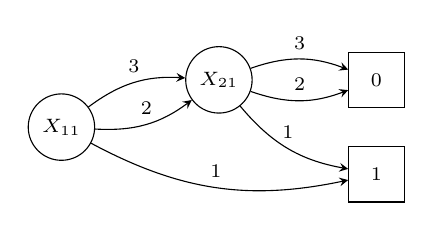
\begin{tikzpicture}
[every node/.style={font=\scriptsize},x=2cm,y=1.2cm,
zeroarrow/.style = {-stealth,dashed},
  onearrow/.style = {-stealth,solid},
  c/.style = {circle,draw,solid,minimum width=2em,
        minimum height=2em},
  r/.style = {rectangle,draw,solid,minimum width=2em,
        minimum height=2em}]
%[place/.style={shape=ellipse}]
%,draw=blue!50,fill=blue!20,thick,inner sep=0pt,minimum size=6mm},

\node[c] (X11) at (0,1) {$X_{11}$};
   \node[c] (X21) at (1,1.5) {$X_{21}$};
   \node[r] (final-one) at (2,0.5) {1};
   \node[r] (final-zero) at (2,1.5){0};

   \path[onearrow,bend right=20] (X11) edge   node [above,midway] {1}(final-one) ;
   \path[onearrow,bend right=20] (X21) edge   node [above,midway] {1}(final-one) ;

   \path[onearrow,bend right=20] (X11) edge   node [above,midway] {2}(X21) ;
   \path[onearrow,bend left=20] (X11) edge   node [above,midway] {3}(X21) ;
   \path[onearrow,bend right=20] (X21) edge   node [above,midway] {2}(final-zero) ;
   \path[onearrow,bend left=20] (X21) edge   node [above,midway] {3}(final-zero) ;
%
%\node (root) at ( 0,1) {};
%\node (node21) at ( 1,1.5){}  ;
%\node (0) at ( 2,1.5) {0};
%\node (1) at ( 2,0.5) {1};
%\path[-,bend left](node21) edge (0) (root) edge node {0} (node21);
%\path[-,bend right]
%			 (root) edge (1)
%(node21) edge (1);
\end{tikzpicture}
\end{center}
}
\newcommand{\mn}{
\begin{center}
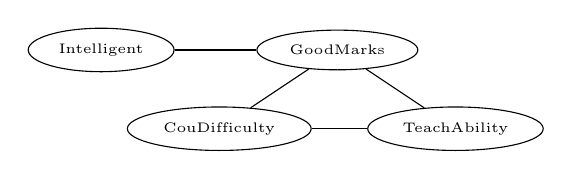
\begin{tikzpicture}
[every node/.style={ellipse,draw,font=\tiny},x=1.5cm,y=1cm]
%[place/.style={shape=ellipse}]
%,draw=blue!50,fill=blue!20,thick,inner sep=0pt,minimum size=6mm},
\node (VisitToAsia) at ( 0,1) {Intelligent};
\node (Tubercolosis) at ( 2,1) [ellipse,draw] {GoodMarks};
\node (Asthma) at ( 1,0) [ellipse,draw] {CouDifficulty};
\node (Cough) at ( 3,0) [ellipse,draw] {TeachAbility};
\path (VisitToAsia) edge  (Tubercolosis)
			 (Tubercolosis) edge (Asthma) edge (Cough)
			(Asthma) edge (Cough);
\end{tikzpicture}\end{center}}

\newcommand{\mln}{
\begin{center}
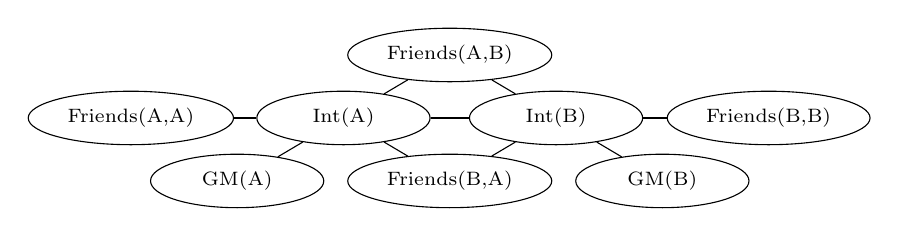
\begin{tikzpicture}
%[every node/.style={ellipse,draw,font=\scriptsize,minimum height=0.5cm,minimum width=2.5cm,
[every node/.style={ellipse,draw,font=\scriptsize,minimum width=2.2cm},x=2.7cm,y=0.8cm]

%[place/.style={shape=ellipse}]
%,draw=blue!50,fill=blue!20,thick,inner sep=0pt,minimum size=6mm},
\node (FriendsAB) at ( 1.5,2) {Friends(A,B)};
\node (FriendsAA) at ( 0,1)  {Friends(A,A)};
\node (FriendsBB) at ( 3,1)  {Friends(B,B)};
\node (FriendsBA) at ( 1.5,0)  {Friends(B,A)};
\node (SmokesA) at ( 1,1)  {Int(A)};
\node (SmokesB) at ( 2,1)  {Int(B)};
\node (CancerA) at ( 0.5,0)  {GM(A)};
\node (CancerB) at ( 2.5,0)  {GM(B)};
\path (FriendsAA) edge  (SmokesA)
		(CancerA) edge (SmokesA)
	(FriendsBB) edge  (SmokesB)
		(CancerB) edge (SmokesB)
	(FriendsAB) edge  (SmokesA)
					edge  (SmokesB)
	(FriendsBA) edge  (SmokesA)
					edge  (SmokesB)
			(SmokesB) edge (SmokesA);

%			 (Tubercolosis) edge (Asthma) edge (Cough)
%			(Asthma) edge (Cough);
\end{tikzpicture}
\end{center}
}


\newcommand{\bn}{
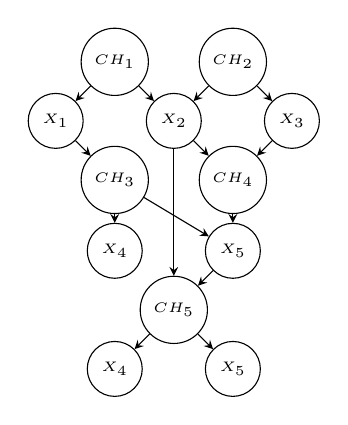
\begin{tikzpicture}
[every node/.style={draw,font=\tiny},x=0.75cm,y=0.75cm,rounded corners=2mm,zeroarrow/.style = {-stealth,dashed},
  onearrow/.style = {-stealth,solid},
  c/.style = {circle,draw,solid},
  r/.style = {rectangle,draw,solid,minimum width=1em,
        minimum height=1em}]
%[place/.style={shape=ellipse}]
%,draw=blue!50,fill=blue!20,thick,inner sep=0pt,minimum size=6mm},

\node[c] (CH1) at (1,5) {$CH_1$};
\node[c] (CH2) at (3,5) {$CH_2$};
\node[c] (X1) at (0,4) {$X_1$};
\node[c] (X2) at (2,4) {$X_2$};
\node[c] (X3) at (4,4) {$X_3$};
\node[c] (CH3) at (1,3) {$CH_3$};
\node[c] (CH4) at (3,3) {$CH_4$};
\node[c] (X4) at (1,1.8) {$X_4$};
\node[c] (X5) at (3,1.8) {$X_5$};
\node[c] (CH5) at (2,0.8) {$CH_5$};
\node[c] (X6) at (1,-0.2) {$X_4$};
\node[c] (X7) at (3,-0.2) {$X_5$};
%
%   \node[c] (X21) at (1,1.5) {#2};
%   \node[r] (final-one) at (2,0.5) {1};
%   \node[r] (final-zero) at (2,1.5){0};
%
%
   \path[onearrow] (CH1) edge (X1) ;
   \path[onearrow] (CH1) edge (X2) ;
   \path[onearrow] (CH2) edge (X2) ;
   \path[onearrow] (CH2) edge (X3) ;
   \path[onearrow] (X1) edge (CH3) ;
   \path[onearrow] (X2) edge (CH4) ;
   \path[onearrow] (X3) edge (CH4) ;
   \path[onearrow] (CH3) edge (X4) ;
   \path[onearrow] (CH3) edge (X5) ;
   \path[onearrow] (CH4) edge (X5) ;
   \path[onearrow] (X2) edge (CH5) ;
   \path[onearrow] (X5) edge (CH5) ;
   \path[onearrow] (CH5) edge (X6) ;
   \path[onearrow] (CH5) edge (X7) ;

%
%%      \draw[onearrow] (X11) -- (final-one);
%%   \draw[onearrow] (X21) -- (final-one);
%
%   \path[zeroarrow,bend left=20] (X11) edge  (X21) ;
%   \path[zeroarrow,bend left=20] (X21) edge  (final-zero) ;
%
%   \draw[zeroarrow] (X11) -- (X21);
%   \draw[zeroarrow] (X21) -- (final-zero);
%
%\node (root) at ( 0,1) {};
%\node (node21) at ( 1,1.5){}  ;
%\node (0) at ( 2,1.5) {0};
%\node (1) at ( 2,0.5) {1};
%\path[-,bend left](node21) edge (0) (root) edge node {0} (node21);
%\path[-,bend right]
%			 (root) edge (1)
%(node21) edge (1);
\end{tikzpicture}
}
%\addtobeamertemplate{background canvas}{\transuncover}{}

\title[PLP - Ch 2 - CC BY 4.0]
{Foundations of Probabilistic Logic Programming}
\subtitle{Chapter 2: Probabilistic Logic Programming Languages}


\author[F. Riguzzi] % (optional, use only with lots of authors)
{Fabrizio Riguzzi}
% - Give the names in the same order as the appear in the paper.
% - Use the \inst{?} command only if the authors have different
%   affiliation.

\institute[] % (optional, but mostly needed)
{
%ENDIF -- University of Ferrara,  Italy\\
% fabrizio.riguzzi@unife.it
}
% - Use the \inst command only if there are several affiliations.
% - Keep it simple, no one is interested in your street address.


\subject{cplint}
% This is only inserted into the PDF information catalog. Can be left
% out.



% If you have a file called "university-logo-filename.xxx", where xxx
% is a graphic format that can be processed by latex or pdflatex,
% resp., then you can add a logo as follows:

\date{}


% Delete this, if you do not want the table of contents to pop up at


% If you wish to uncover everything in a step-wise fashion, uncomment
% the following command:

%\beamerdefaultoverlayspecification{<+->}
%\AtBeginSection[]
%{
%\begin{frame}
%\frametitle{Outline}
%\end{frame}
%}
\begin{document}
\begin{frame}
\titlepage
\vspace{-2cm}
\begin{center}
\includegraphics[scale=0.120]{plp-book.jpg}

\includegraphics[scale=0.3]{cc-by.png}

\end{center}
\end{frame}



\begin{frame}
  \frametitle{Outline}
\begin{itemize}
\item Probabilistic logic programming
\item Applications
\item Exact inference
\end{itemize}
\end{frame}

\begin{frame}
  \frametitle{Combining Logic and Probability}
\begin{itemize}
\item Logic does not handle well uncertainty
\item Graphical models do not handle well relationships among entities
\item Solution: combine the two
\item Many approaches proposed in the areas of Logic Programming, Uncertainty in AI, Machine Learning, Databases, Knowledge Representation
\end{itemize}
\end{frame}
\begin{frame}
  \frametitle{Probabilistic Logic Programming}
\begin{itemize}
\item Distribution Semantics [Sato ICLP95]%\cite{DBLP:conf/iclp/Sato95}
\item A probabilistic logic program defines a probability distribution over normal logic programs (called \myalert{instances} or \myalert{possible worlds} or simply \myalert{worlds})
\item The distribution is extended to a joint distribution over worlds and interpretations (or queries)
\item The probability of a query is obtained from this distribution
\end{itemize}
\end{frame}


\begin{frame}
  \frametitle{Probabilistic Logic Programming (PLP) Languages under the Distribution Semantics}
\begin{itemize}
\item Probabilistic Logic Programs [Dantsin RCLP91]%\cite{DBLP:conf/lpar/Dantsin91}
\item Probabilistic Horn Abduction [Poole NGC93],
%\cite{DBLP:journals/ngc/Poole93},
Independent Choice Logic (ICL) [Poole AI97]%\cite{Poo97-ArtInt-IJ}
\item PRISM [Sato ICLP95]%\cite{DBLP:conf/iclp/Sato95}
\item Logic Programs with Annotated Disjunctions (LPADs) [Vennekens et al. ICLP04]%\cite{VenVer04-ICLP04-IC}
\item ProbLog [De Raedt et al. IJCAI07]%\cite{DBLP:conf/ijcai/RaedtKT07}
\item They differ in the way they define the distribution over logic programs
\end{itemize}
\end{frame}


\begin{frame}
  \frametitle{Logic Programs with Annotated Disjunctions}
  \url{http://cplint.eu/e/sneezing_simple.pl}
 $$\begin{array}{l}
sneezing(X):0.7 \orh null:0.3\leftarrow \mathit{flu}(X).\\
sneezing(X):0.8\orh null:0.2\leftarrow hay\_\mathit{fever}(X).\\
\mathit{flu}(bob).\\
hay\_\mathit{fever}(bob).\\
 \end{array}$$
\begin{itemize}
\item Distributions over the head of rules
\item $null$ does not appear in the body of any rule
\item Worlds obtained by selecting one atom from the head of every grounding of each clause
\end{itemize}
\end{frame}

\begin{frame}
  \frametitle{Distribution Semantics}
\begin{itemize}
\item Case of no function symbols: finite Herbrand universe, finite set of groundings of each disjoint statement/switch/clause
\item \myalert{Atomic choice}: selection of the $i$-th atom for grounding $C\theta$ of switch/clause $C$
\begin{itemize}
\item represented with the triple $(C,\theta,i)$
\end{itemize}
\item Example $C_1=sneezing(X):0.7\orh null:0.3\leftarrow \mathit{flu}(X).$,
$(C_1,\{X/bob\},1)$
\end{itemize}
\end{frame}

\begin{frame}
  \frametitle{Distribution Semantics}
\begin{itemize}
\item \myalert{Selection} $\sigma$: a total set of atomic choices (one atomic choice
for every grounding of each clause)
\item A selection $\sigma$ identifies a  logic program $w_\sigma$ called  \myalert{world}
\item The probability of $w_\sigma$ is $P(w_\sigma)=\prod_{(C,\theta,i)\in \sigma}P_0(C,i)$
\item Finite set of worlds: $W_T=\{w_1,\ldots,w_m\}$
\item $P(w)$ distribution over worlds:  $\sum_{w\in W_T}P(w)=1$
\end{itemize}
\end{frame}
\begin{frame}
  \frametitle{Distribution Semantics}
\begin{itemize}
\item Ground query $Q$
\item $P(Q|w)=1$ if $Q$ is true in $w$ and 0 otherwise
\item $P(Q)=\sum_{w}P(Q,w)=\sum_{w}P(Q|w)P(w)=\sum_{w\models Q}P(w)$
\end{itemize}
\end{frame}


\begin{frame}
  \frametitle{Example Program (LPAD) Worlds}
  \url{http://cplint.eu/e/sneezing_simple.pl}
\begin{footnotesize}
$$ \begin{array}{ll}
 sneezing(bob)\leftarrow \mathit{flu}(bob).& null\leftarrow \mathit{flu}(bob).\\
 sneezing(bob)\leftarrow hay\_\mathit{fever}(bob).& sneezing(bob)\leftarrow hay\_\mathit{fever}(bob).\\
\mathit{flu}(bob).&\mathit{flu}(bob).\\
 hay\_\mathit{fever}(bob).&hay\_\mathit{fever}(bob).\\
P(w_1)=0.7\times 0.8 &P(w_2)=0.3\times 0.8\\
\\
 sneezing(bob)\leftarrow \mathit{flu}(bob).& null\leftarrow \mathit{flu}(bob).\\
 null\leftarrow hay\_\mathit{fever}(bob).& null\leftarrow hay\_\mathit{fever}(bob).\\
\mathit{flu}(bob).&\mathit{flu}(bob).\\
 hay\_\mathit{fever}(bob). &hay\_\mathit{fever}(bob).\\
P(w_3)=0.7\times 0.2 &P(w_4)=0.3\times 0.2
 \end{array}$$
\begin{equation*}
\label{ds}
P(Q)=\sum_{w\in W_\mathcal{T}}P(Q,w)=\sum_{w \in W_\mathcal{T}}P(Q|w)P(w)=\sum_{w\in W_\mathcal{T}: w\models Q}P(w)
\end{equation*}
\end{footnotesize}
\begin{itemize}
\item $sneezing(bob)$ is true in 3 worlds
\item $P(sneezing(bob))=0.7\times 0.8+0.3\times 0.8+0.7\times 0.2=0.94$
\end{itemize}
\end{frame}

\begin{frame}
  \frametitle{Logic Programs with Annotated Disjunctions}
  \url{http://cplint.eu/e/sneezing.pl}
\begin{footnotesize}
 $$\begin{array}{l}
strong\_sneezing(X):0.3\orh moderate\_sneezing(X):0.5\leftarrow \mathit{flu}(X).\\
strong\_sneezing(X):0.2\orh moderate\_sneezing(X):0.6\leftarrow hay\_\mathit{fever}(X).\\
\mathit{flu}(bob).\\
hay\_\mathit{fever}(bob).\\
 \end{array}$$
\end{footnotesize}
\begin{itemize}
\item 9 worlds
\item $strong\_sneezing(bob))$ is true in 5
\item $P(strong\_sneezing(bob))=0.3\cdot 0.2+0.3\cdot 0.6+0.3\cdot 0.2+0.5\cdot 0.2+0.2\cdot 0.2=0.44$
\end{itemize}
\end{frame}


\begin{frame}[fragile]
  \frametitle{Applications}
\begin{itemize}
\item Link prediction: given a (social) network, compute the probability of the existence of a link between two
entities (UWCSE)
  \end{itemize}
\begin{center}
\includegraphics[width=0.35\textwidth]{social.png}
\end{center}
\begin{verbatim}
advisedby(X, Y) :0.7 :-
  publication(P, X),
  publication(P, Y),
  student(X).
\end{verbatim}
\begin{tiny}
Image by Zigomitros Athanasios, CC BY-SA 3.0, \url{https://commons.wikimedia.org/wiki/File:Social_Network.png}
\end{tiny}
\end{frame}
\begin{frame}[fragile]
  \frametitle{Applications}
\begin{itemize}
\item Classify web pages on the basis of the link structure (WebKB)
  \end{itemize}
	\begin{center}
\includegraphics[scale=0.18]{800px-WorldWideWebAroundWikipedia.png}
\end{center}
\begin{scriptsize}
\begin{verbatim}
coursePage(Page1): 0.3 :- linkTo(Page2,Page1),coursePage(Page2).
coursePage(Page1): 0.6 :- linkTo(Page2,Page1),facultyPage(Page2).
...
coursePage(Page): 0.9 :- has('syllabus',Page).
...
\end{verbatim}
\end{scriptsize}
\begin{tiny}
Image by Chris 73, CC BY-SA 3.0, \url{https://en.wikipedia.org/wiki/File:WorldWideWebAroundWikipedia.png}
\end{tiny}

\end{frame}

\begin{frame}[fragile]
  \frametitle{Applications}
\begin{itemize}
\item Entity resolution: identify identical entities in text or databases
  \end{itemize}
	\begin{columns}
	\begin{column}{0.5\textwidth}
\begin{center}
\includegraphics[scale=0.3]{entity-res.png}
\end{center}
\end{column}
\begin{column}{0.5\textwidth}
\begin{tiny}
\begin{verbatim}
samebib(A,B):0.9 :-
	samebib(A,C), samebib(C,B).
sameauthor(A,B):0.6 :-
  sameauthor(A,C), sameauthor(C,B).
sametitle(A,B):0.7 :-
  sametitle(A,C), sametitle(C,B).
samevenue(A,B):0.65 :-
  samevenue(A,C), samevenue(C,B).
samebib(B,C):0.5 :-
  author(B,D),author(C,E),sameauthor(D,E).
samebib(B,C):0.7 :-
  title(B,D),title(C,E),sametitle(D,E).
samebib(B,C):0.6 :-
  venue(B,D),venue(C,E),samevenue(D,E).
samevenue(B,C):0.3 :-
  haswordvenue(B,logic),
  haswordvenue(C,logic).
...
\end{verbatim}
\end{tiny}
\end{column}
\end{columns}
\begin{tiny}
Image from \url{http://www.datacommunitydc.org/blog/2013/08/entity-resolution-for-big-data}
\end{tiny}

\end{frame}

\begin{frame}[fragile]
  \frametitle{Applications}
\begin{itemize}
\item Chemistry: given the chemical composition of a substance, predict its mutagenicity or its carcenogenicity
  \end{itemize}
		\begin{columns}
	\begin{column}{0.5\textwidth}
\begin{center}
\includegraphics[scale=0.425]{mutagens.png}
\end{center}
\end{column}
\begin{column}{0.5\textwidth}
\begin{footnotesize}
\begin{verbatim}
active(A):0.4 :-
   atm(A,B,c,29,C),
   gteq(C,-0.003),
   ring_size_5(A,D).
active(A):0.6:-
   lumo(A,B), lteq(B,-2.072).
active(A):0.3 :-
   bond(A,B,C,2),
   bond(A,C,D,1),
   ring_size_5(A,E).
active(A):0.7 :-
   carbon_6_ring(A,B).
active(A):0.8 :-
   anthracene(A,B).
...
\end{verbatim}
\end{footnotesize}
\end{column}
\end{columns}
\begin{tiny}
Image from \url{https://www.doc.ic.ac.uk/~shm/mutagenesis.html}
\end{tiny}

\end{frame}

\begin{frame}
  \frametitle{Applications}
\begin{itemize}
\item Medicine: diagnose diseases on the basis of patient information (Hepatitis), influence of genes on HIV, risk of falling of elderly people
  \end{itemize}

\end{frame}

%\begin{frame}
%  \frametitle{Weight Learning}
%
%  \begin{itemize}
%		\item Given
%  \begin{itemize}
%		\item model: a probabilistic logic model with unknown parameters
%		\item data: a set of interpretations
%  \end{itemize}
%  \item Find the values of the parameters that maximize the probability of the data given the model
%  \item Discriminative learning: maximize the conditional probability of a set of outputs (e.g. ground instances for a predicate) given a set of inputs
%  \item Alternatively, the data are  queries for which we know the probability: minimize the error in the probability of the queries that is returned by the model
%  \end{itemize}
%\end{frame}
%
%\begin{frame}
%  \frametitle{Structure Learning}
%
%  \begin{itemize}
%		\item Given
%  \begin{itemize}
%		\item language bias: a specification of the search space
%		\item data: a set of interpretations
%  \end{itemize}
%  \item Find the formulas and the parameters that maximize the likelihood of the data given the model
%  \item Discriminative learning: again maximize the conditional likelihood of a set of outputs  given a set of inputs
%  \end{itemize}
%\end{frame}
%



\begin{frame}
  \frametitle{Inference for PLP under DS}

  \begin{itemize}
  \item Computing the probability of a query (no evidence)
		\item Knowledge compilation:
  	\begin{itemize}
  		\item compile the program to an intermediate representation
  		\begin{itemize}
  			\item    Binary Decision Diagrams (ProbLog [De Raedt et al. IJCAI07], \texttt{cplint} [Riguzzi AIIA07,Riguzzi LJIGPL09], PITA [Riguzzi \& Swift ICLP10])
				%				\cite{Rig-AIIA07-IC,Rig09-LJIGPL-IJ}, PITA \cite{RigSwi10-ICLP10-IC})
  			\item deterministic, Decomposable Negation Normal Form circuit (d-DNNF) (ProbLog2 [Fierens et al. TPLP15])
%				\cite{DBLP:journals/corr/abs-1304-6810})
				\item Sentential Decision Diagrams
  		\end{itemize}
  		\item compute the probability by weighted model counting
  	\end{itemize}
  \end{itemize}
\end{frame}
%



\begin{frame}
  \frametitle{Inference for PLP under DS}

  \begin{itemize}
  	\item Bayesian Network  based:
  \begin{itemize}
  \item Convert to BN
  \item Use BN inference algorithms (CVE [Meert et al. ILP09])
%	\cite{MeeStrBlo08-ILP09-IC})
  \end{itemize}
  \item Lifted inference
  \end{itemize}
\end{frame}


\begin{frame}[fragile]
  \frametitle{Examples}
Throwing coins \url{http://cplint.eu/e/coin.swinb}
\begin{verbatim}
heads(Coin):1/2 ; tails(Coin):1/2 :-
  toss(Coin),\+biased(Coin).
heads(Coin):0.6 ; tails(Coin):0.4 :-
  toss(Coin),biased(Coin).
fair(Coin):0.9 ; biased(Coin):0.1.
toss(coin).
\end{verbatim}
Russian roulette with two guns \url{http://cplint.eu/e/trigger.pl}
\begin{verbatim}
death:1/6 :- pull_trigger(left_gun).
death:1/6 :- pull_trigger(right_gun).
pull_trigger(left_gun).
pull_trigger(right_gun).
\end{verbatim}
\end{frame}

\begin{frame}[fragile]
  \frametitle{Examples}
Mendel's inheritance rules for pea plants \url{http://cplint.eu/e/mendel.pl}
\begin{verbatim}
color(X,purple):-cg(X,_A,p).
color(X,white):-cg(X,1,w),cg(X,2,w).
cg(X,1,A):0.5 ; cg(X,1,B):0.5 :-
  mother(Y,X),cg(Y,1,A),cg(Y,2,B).
cg(X,2,A):0.5 ; cg(X,2,B):0.5 :-
  father(Y,X),cg(Y,1,A),cg(Y,2,B).
\end{verbatim}
Probability of paths \url{http://cplint.eu/e/path.swinb}
\begin{verbatim}
path(X,X).
path(X,Y):-path(X,Z),edge(Z,Y).
edge(a,b):0.3.
edge(b,c):0.2.
edge(a,c):0.6.
\end{verbatim}
\end{frame}

%\begin{frame}[fragile]
%  \frametitle{Encoding Bayesian Networks}
%%\begin{columns}[t]
%
%%\begin{column}{0.65\textwidth}
%\begin{center}
%
%\begin{tikzpicture}
%[c/.style={ellipse,draw,font=\scriptsize,minimum height=0.5cm,minimum width=2.5cm},x=2cm,y=1.2cm]
%%[place/.style={shape=ellipse}]
%%,draw=blue!50,fill=blue!20,thick,inner sep=0pt,minimum size=6mm},
%\node[c] (burg) at ( 0,1) {Burglary};
%\node[c] (earthq) at ( 2,1)  {Earthquake};
%\node[c] (alarm) at ( 1,0) {Alarm};
%\node (tab) at (4,0.5) {\begin{tabular}{|c|c|c|}
%\hline
%alarm&t &f \\\hline
%b=t,e=t&1.0&0.0\\\hline
%b=t,e=f&0.8&0.2\\\hline
%b=f,e=t&0.8&0.2\\\hline
%b=f,e=f&0.1&0.9\\\hline
%\end{tabular}};
%
%\node at (2,-1){
%\begin{tabular}{|c|c|c|}
%\hline
%burg&t &f \\\hline
%&0.1&0.9\\\hline
%\end{tabular}
%\begin{tabular}{|c|c|c|}
%\hline
%earthq&t &f \\\hline
%&0.2&0.8\\\hline
%\end{tabular}
%};
%\path[->] (burg) edge  (alarm)
%			 (earthq) edge (alarm);
%\end{tikzpicture}
%\end{center}
%%\end{column}
%%\begin{column}{0.35\textwidth}
%%
%%\begin{tabular}{|c|c|c|}
%%\hline
%%alarm&t &f \\\hline
%%b=t,e=t&1.0&0.0\\\hline
%%b=t,e=f&0.8&0.2\\\hline
%%b=f,e=t&0.8&0.2\\\hline
%%b=f,e=f&0.1&0.9\\\hline
%%\end{tabular}
%%
%%\begin{tabular}{|c|c|c|}
%%\hline
%%burg&t &f \\\hline
%%&0.1&0.9\\\hline
%%\end{tabular}
%%\begin{tabular}{|c|c|c|}
%%\hline
%%earthq&t &f \\\hline
%%&0.2&0.8\\\hline
%%\end{tabular}
%%
%%
%%\end{column}
%%\end{columns}
%\begin{footnotesize}
%\begin{verbatim}
%burg(t):0.1 ; burg(f):0.9.
%earthq(t):0.2 ; earthq(f):0.8.
%alarm(t):-burg(t),earthq(t).
%alarm(t):0.8 ; alarm(f):0.2:-burg(t),earthq(f).
%alarm(t):0.8 ; alarm(f):0.2:-burg(f),earthq(t).
%alarm(t):0.1 ; alarm(f):0.9:-burg(f),earthq(f).
%\end{verbatim}
%\end{footnotesize}
%
%\end{frame}
\begin{frame}
  \frametitle{PLP Online}
\begin{itemize}
\item
\url{http://cplint.eu}
\begin{itemize}
\item Inference (knwoledge compilation, Monte Carlo)
\item Parameter learning (EMBLEM)
\item Structure learning (SLIPCOVER, LEMUR)
\end{itemize}
\end{itemize}
\end{frame}

\begin{frame}[fragile]
  \frametitle{Epidemic Example}

If somebody has the flu and the climate is cold, an epidemic arises with 60\% probability, a pandemic arises with 30\% probability, whereas we have a 10\% probability that neither an epidemic nor a pandemic arises. We can write
\begin{scriptsize}
\begin{verbatim}
epidemic : 0.6; pandemic : 0.3; null: 0.1 :- flu(_), cold.
\end{verbatim}
\end{scriptsize}
The null atom can be implicit. Therefore the previous rule, without changing its meaning, can be written
\begin{scriptsize}
\begin{verbatim}
epidemic : 0.6; pandemic : 0.3 :- flu(_), cold.
\end{verbatim}
\end{scriptsize}
\end{frame}

\begin{frame}[fragile]
  \frametitle{Epidemic Example}

The weather is cold with a 70\% probability. Note that the null atom is implicit here as well.
\begin{scriptsize}
\begin{verbatim}
cold : 0.7.
\end{verbatim}
\end{scriptsize}
David and Robert have the flu for certain:
\begin{scriptsize}
\begin{verbatim}
flu(david).
flu(robert).
\end{verbatim}
\end{scriptsize}
\end{frame}

\begin{frame}[fragile]
  \frametitle{Epidemic Example}
The program is almost complete,  we need  to load the library pita in order to perform exact inference
\begin{scriptsize}
\begin{verbatim}
:- use_module(library(pita)).
\end{verbatim}
\end{scriptsize}
We need to initalize the library with \verb|:-pita| and the program should be enclosed by \verb|:- begin_lpad.| and \verb|:- end_lpad.| (respectively at the begin and at the end of the program). 
\end{frame}
\begin{frame}[fragile]
  \frametitle{Epidemic Example}
\begin{verbatim}
:- use_module(library(pita)).
:- pita.
:- begin_lpad.
epidemic : 0.6; pandemic : 0.3 :- flu(_), cold.
cold : 0.7.
flu(david).
flu(robert).
:- end_lpad.
\end{verbatim}
\end{frame}

\begin{frame}[fragile]
  \frametitle{How to Execute a Simple Query}

To query a program you must use the \verb|prob/2| predicate
\begin{verbatim}
prob(:Query:atom,-Probability:float).
\end{verbatim}
 Let us compute the probability that an epidemic arises:
\begin{verbatim}
prob(epidemic, P).
\end{verbatim}
You can ask conditional queries with 
\begin{verbatim}
prob(:Query:atom,:Evidence:atom,-Probability:float).
\end{verbatim}
Remember: $P(q|e)=\frac{P(q,e)}{P(e)}$

We can ask for the probability that an epidemic arises given that outside is cold
\begin{verbatim}
prob(epidemic, cold, P).
\end{verbatim}
\end{frame}
\begin{frame}
  \frametitle{Monty Hall Puzzle}
\begin{itemize}
\item A player is given the opportunity to
select one of three closed doors, behind one of which there is a prize.
\item Behind the other two doors are empty rooms.
\item
Once the player has made a selection, Monty is obligated to open one of the
remaining closed doors which does not contain the prize, showing that the room
behind it is empty.
\item He then asks the player if he would like to switch
his selection to the other unopened door, or stay with his original choice.
\item Does it matter if he switches?
\end{itemize}
\end{frame}
\begin{frame}[fragile]
  \frametitle{Monty Hall Puzzle}
\begin{scriptsize}
\begin{verbatim}
:- use_module(library(pita)).
:- endif.
:- pita.
:- begin_lpad.
prize(1):1/3; prize(2):1/3; prize(3):1/3.

open_door(2):0.5 ; open_door(3):0.5:- prize(1).
open_door(2):- prize(3).
open_door(3):- prize(2).

win_keep:- prize(1).

win_switch:-
  prize(2),
  open_door(3).

win_switch:-
  prize(3),
  open_door(2).
:- end_lpad.
\end{verbatim}
\end{scriptsize}
\end{frame}

\begin{frame}[fragile]
  \frametitle{Monty Hall Puzzle}
\begin{itemize}
\item Queries:
\end{itemize}
\begin{verbatim}
prob(win_keep,Prob).
prob(win_switch,Prob).
\end{verbatim}
\end{frame}


\begin{frame}[fragile]
  \frametitle{Game of dice}
    \begin{verbatim}
on(0,1):1/3 ; on(0,2):1/3 ; on(0,3):1/3.
on(T,1):1/3 ; on(T,2):1/3 ; on(T,3):1/3 :-
  T1 is T-1, T1>=0, on(T1,F), \+ on(T1,3).
\end{verbatim}

  
What is the probability that the die lands on face 1 at time 2?
  \begin{verbatim}
?- prob(on(2,1),Prob).
\end{verbatim}
What is the probability that the die lands on face 1 at time 2 given that it landed on face 1 at time 0?
  \begin{verbatim}
?- prob(on(2,1),on(0,1),Prob).
\end{verbatim}
\end{frame}

%\begin{frame}[fragile]
%\frametitle{Hidden Markov Models}
%\begin{center}
%\begin{tikzpicture}[
%%every node/.style={ellipse,draw,font=\scriptsize,minimum height=0.5cm,minimum width=1.8cm
%%},
%x=2.5cm,y=1cm]
%%[place/.style={shape=ellipse}]
%%,draw=blue!50,fill=blue!20,thick,inner sep=0pt,minimum size=6mm},
%\node [font=\tiny] (xtm2) at ( -1,1) {$\ldots$};
%\node
%[ellipse,draw,font=\tiny,minimum height=0.35cm,minimum width=1.5cm,font=\tiny]
%(xtm1) at ( 0,1) {$X(t-1)$};
%\node (xt0)
%[ellipse,draw,font=\tiny,minimum height=0.35cm,minimum width=1.5cm,font=\tiny]
% at ( 1,1) {$X(t)$};
%\node (xtp1)
%[ellipse,draw,font=\tiny,minimum height=0.35cm,minimum width=1.5cm,font=\tiny]
%at ( 2,1) {$X(t+1)$};
%\node [font=\tiny] (xtp2) at ( 3,1) {$\ldots$};
%\node
%[ellipse,draw,font=\tiny,minimum height=0.35cm,minimum width=1.5cm,font=\tiny]
%(ytm1) at ( 0,0) {$Y(t-1)$};
%\node
%[ellipse,draw,font=\tiny,minimum height=0.35cm,minimum width=1.5cm,font=\tiny]
%(yt0) at ( 1,0) {$Y(t)$};
%\node
%[ellipse,draw,font=\tiny,minimum height=0.35cm,minimum width=1.5cm,font=\tiny]
% (ytp1) at ( 2,0) {$Y(t+1)$};
%\path[->] (xtm2) edge  (xtm1)
%(xtm1) edge  (xt0) edge (ytm1)
% (xt0) edge  (xtp1) edge (yt0)
%  (xtp1) edge   (ytp1)
%   (xtp1) edge  (xtp2) ;
%  \end{tikzpicture}
%\end{center}
%\begin{scriptsize}
%\begin{verbatim}
%hmm(S,O):-hmm(q1,[],S,O).
%hmm(end,S,S,[]).
%hmm(Q,S0,S,[L|O]):-
%  Q\= end,
%  next_state(Q,Q1,S0),
%  letter(Q,L,S0),
%  hmm(Q1,[Q|S0],S,O).
%next_state(q1,q1,_S):1/3;next_state(q1,q2_,_S):1/3;
%  next_state(q1,end,_S):1/3.
%next_state(q2,q1,_S):1/3;next_state(q2,q2,_S):1/3;
%  next_state(q2,end,_S):1/3.
%letter(q1,a,_S):0.25;letter(q1,c,_S):0.25;
%  letter(q1,g,_S):0.25;letter(q1,t,_S):0.25.
%letter(q2,a,_S):0.25;letter(q2,c,_S):0.25;
%  letter(q2,g,_S):0.25;letter(q2,t,_S):0.25.
%\end{verbatim}
%\end{scriptsize}
%\end{frame}
\begin{frame}[fragile]
  \frametitle{Graphics}
cplint on SWISH can show the probabilistic results of a query as histograms using predicate \verb|bar/2|
\begin{verbatim}
bar(+Probability:float,-Chart:dict).
\end{verbatim}
A graphical bar chart of the two values will be plotted

Examples:
\begin{verbatim}
prob(epidemic, P),bar(P,G).
prob(epidemic, cold, P),bar(P,G).
\end{verbatim}
\end{frame}

\end{document}


